\chapter{Photons generation in coupled resonators}
\begin{figure}
\centering
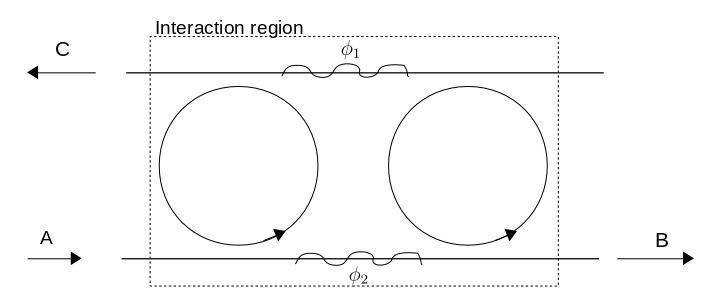
\includegraphics[width = \textwidth]{img/system}
\caption{Coupled resonators, Spontaneous Four wave mixing happens only inside the rings, there are three channel labelled as A,B and C}
\label{couplesstructure}
\end{figure}

In this last chapter we study the generation of entangled photons via Spontaneous Four Wave Mixing in the structure of figure \ref{couplesstructure}. The work starts by writing the non linear Hamiltonian in terms of the asymptotic states developed in section \ref{section:asymptotic}, then we solve the dynamics of the photons state using the backward Heinsenberg approch developed in section \ref{heinsemberg} and finally we study the results.\\
\section{Output state}
We take as input state a coherent state in channel A, so we can write it as $\ket{\psi_{in}} = e^{\alpha A_p^\dagger - \text{H.c}}\ket{vac}$ where $A_p^\dagger = \int dk \phi_P(k) a_k^\dagger$. The non linear Hamiltonian is []
\begin{equation}\label{nonlinearhamiltonian}H_{NL} = -\frac{1}{3\varepsilon_0}\int\Gamma^{ijkl}_3(\r)D^iD^jD^kD^l\,d\r\end{equation}
where the summation over repeated indexes is implicit. A natural choice is to write the displacement operator associated with channel $A$ in terms of the asymptotic-in fields, and the operator for channel $B$ and $C$ in terms of the asymptotic-out fields. So we can write the displacement operator as:
\begin{equation}\mathbf{D}(\r) = \int_0^{+\infty}dk\sqrt{\frac{\hbar\omega_k}{2}}\left[a_{k}\mathbf{D}^{asy-in}_{a,k}(\r)+b_{b,k}\mathbf{D}^{asy-out}_{b,k}(\r)+b_{c,k}\mathbf{D}^{asy-out}_{c,k}(\r)\right] +\text{H.c.}\end{equation}
where $a_k$ is the annihilation operator associated with channel A, $b_{b,k}$ is for channel B and $b_{c,k}$ refers to channel C. Putting this inside expression \eqref{nonlinearhamiltonian} and keeping only the Spontaneous Four Wave Mixing terms we arrive at:
\begin{multline}H_{NL} = -\int dk_1dk_2dk_3dk_4S_{bb}(k_1,k_2,k_3,k_4)a_{k_1}a_{k_2}b_{b,k_3}^\dagger b_{b,k_4}^\dagger \\-2\int dk_1dk_2dk_3dk_4S_{bc}(k_1,k_2,k_3,k_4)a_{k_1}a_{k_2}b_{b,k_3}^\dagger b_{c,k_4}^\dagger\\ -\int dk_1dk_2dk_3dk_4S_{cc}(k_1,k_2,k_3,k_4)a_{k_1}a_{k_2}b_{c,k_3}^\dagger b_{c,k_4}^\dagger +\text{H.c.}\end{multline}
where we defined the following quantity
\begin{multline}\label{S}
S_{xy}(k_1,k_2,k_3,k_4) = \frac{3}{2\varepsilon_0}\sqrt{\frac{(\hbar\omega_{k_1})(\hbar\omega_{k_2})(\hbar\omega_{k_3})(\hbar\omega_{k_4})}{16}}\cdot \\ \int d\r \Gamma^{ijkl}_3D^{i,asy-in}_{a,k_1}(\r)D^{j,asy-in}_{a,k_2}(\r)\left[D^{k,asy-out}_{x,k_3}(\r)\right]^*\left[D^{l,asy-out}_{y,k_4}(\r)\right]^*
\end{multline}
with this expression in hands we can switch to the Heisenberg picture e we can define
\begin{equation}\label{potential}
V(t) = U_L^\dagger H_{NL}U_{L}\end{equation}
since the operator $U_L$ satisfies the unitary relation $U_L U_L^\dagger = U_L^\dagger U_L = \mathbbm{1}$ we can isert $U_L^\dagger U_L$ between every annhilation and creation operators and define the time dependent operators, for example $a_{k}(t) \equiv U_L^\dagger a_{k}U_L$. Time dependent operators satisfies the Heisenberg equation
\begin{equation}\frac{da_{k}}{dt} = \frac{1}{i\hbar}[a_{k},H_L]\end{equation}
which we can solve for every operators. For example for $a_{k}$ the commutator with the linear Hamiltonian is:
\begin{equation}[a_{k},H_L] = \int dk'\hbar \omega_{k'}a_{k} a_{k'}^\dagger a_{k'}-\int dk'\hbar \omega_{k'}a_{k'}^\dagger a_{k'}a_{k}\end{equation}
we know that $[a_k,a_{k'}^\dagger] = \delta(k-k')\implies a_{k} a_{k'}^\dagger = \delta(k-k') + a_{k'}^\dagger a_{k}$ substituting this into the first term we arrive at
\begin{equation}[a_{k},H_L] = \int dk'\hbar \omega_{k'}a_{k}\delta(k-k') = \hbar \omega_{k}a_{k}\end{equation}
so the Heisenberg equation can be written as
\begin{equation}\frac{da_{k}}{dt} = -i\omega_{k}a_{k}\end{equation}
which has the trivial solution $a_k(t) = a_k(0)e^{-i\omega_k t}$, since $a_k(0) = a_k$ we can write \eqref{potential} 
\begin{equation}V(t) = V_{bb} + 2V_{bc} + V_{cc}\end{equation}
where
\begin{equation}V_{xy} = -\int dk_1dk_2dk_3dk_4S_{xy}(k_1,k_2,k_3,k_4;t)a_{k_1}a_{k_2}b_{x,k_3}^\dagger b_{y,k_4}^\dagger +\text{H.c} \end{equation}
and $S_{xy}(k_1,k_2,k_3,k_4;t) = S_{xy}(k_1,k_2,k_3,k_4)e^{-i(\omega_{k1}+\omega_{k2}-\omega_{k3}-\omega_{k4})t}$. In a similar way it's possible to construct $\hat{V}(t)$
\begin{equation}\hat{V}(t) = U(t_1,t)V(t)U^\dagger(t_1,t) = \hat{V}_{bb}(t) + 2\hat{V}_{bc}(t) + \hat{V}_{cc}(t)\end{equation}
where 
\begin{equation}\hat{V}_{xy}(t) = -\int dk_1dk_2dk_3dk_4S_{xy}(k_1,k_2,k_3,k_4;t)\overline{a}_{k_1}(t)\overline{a}_{k_2}(t)\overline{b}_{x,k_3}^\dagger(t) \overline{b}_{y,k_4}^\dagger(t) +\text{H.c}\end{equation}
now we have all the elements for integrating the equation \eqref{dynamicO}, we need to solve it for the operator $\overline{a}^\dagger_{k}(t)$
\begin{equation}\label{meinkampf}-i\hbar \frac{d\overline{a}^\dagger_{k}(t)}{dt} = [\overline{a}^\dagger_{k},\hat{V}(t)] = [\overline{a}^\dagger_{k},\hat{V}_{bb}(t)] + [\overline{a}^\dagger_{k},2\hat{V}_{bc}(t)] +[\overline{a}^\dagger_{k},\hat{V}_{cc}(t)]\end{equation}
we need to work out the three commutator, they are all  similar, so we show only one
\begin{multline}[\overline{a}^\dagger_{k},\hat{V}_{bb}(t)] = -\int dk_1dk_2dk_3dk_4S_{bb}(k_1,k_2,k_3,k_4;t)\overline{a}^\dagger_{k}(t)\overline{a}_{k_1}(t)\overline{a}_{k_2}(t)\overline{b}_{b,k_3}^\dagger(t) \overline{b}_{b,k_4}^\dagger(t) \\
-\int dk_1dk_2dk_3dk_4S_{bb}(k_1,k_2,k_3,k_4;t)\overline{a}^\dagger_{k}(t)\overline{a}^\dagger_{k_1}(t)\overline{a}^\dagger_{k_2}(t)\overline{b}_{b,k_3}(t) \overline{b}_{b,k_4}(t) \\
+ \int dk_1dk_2dk_3dk_4S_{bb}(k_1,k_2,k_3,k_4;t)\overline{a}_{k_1}(t)\overline{a}_{k_2}(t)\overline{b}_{b,k_3}^\dagger(t) \overline{b}_{b,k_4}^\dagger(t)\overline{a}^\dagger_{k}(t)\\ 
+ \int dk_1dk_2dk_3dk_4S_{bb}(k_1,k_2,k_3,k{}_4;t)\overline{a}^\dagger_{k}(t)\overline{a}^\dagger_{k_1}(t)\overline{a}^\dagger_{k_2}(t)\overline{b}_{b,k_3}(t) \overline{b}_{b,k_4}\overline{a}^\dagger_{k}(t) \end{multline}
the second and the fourth term are indentical, therefore they can be eliminated, for the first one we can use \eqref{acommutator}, at the end we get
\[[\overline{a}^\dagger_{k},\hat{V}_{bb}(t)] = 2\int dk_1 dk_2 dk_3 S_{bb}(k_1,k_2,k_3,k,t)\overline{a}_{k_1}(t)\overline{b}_{b,k_2}^\dagger(t)\overline{b}_{b,k_3}^\dagger(t)\]
the zeroth-order solution of \eqref{meinkampf} is $\overline{a}^\dagger_{k}(t) = \overline{a}^\dagger_{k}(t_1) = a_k^\dagger$, so, the first order solution is
\begin{multline}\label{abarra}\overline{a}^\dagger_{k}(t) = a_k^\dagger + \frac{2}{i\hbar}\int dk_1dk_2 dk_3 \int_{t_1}^tS_{bb}(k_1,k_2,k_3,k,t)a_{k_1}b_{b,k_2}^\dagger b_{b,k_3}^\dagger \\+\frac{4}{i\hbar}\int dk_1dk_2 dk_3 \int_{t_1}^tS_{bc}(k_1,k_2,k_3,k,t)a_{k_1}b_{b,k_2}^\dagger b_{c,k_3}^\dagger \\
+ \frac{2}{i\hbar}\int dk_1dk_2 dk_3 \int_{t_1}^tS_{cc}(k_1,k_2,k_3,k,t)a_{k_1}b_{c,k_2}^\dagger b_{c,k_3}^\dagger \end{multline}
with this expression we can write the output state as
\[\ket{\psi_{out}} = e^{\alpha \overline{A}_P^\dagger(t_0)-\text{H.c}}\]
where $\overline{A}_P^\dagger(t_0) = \int dk \phi_P(k)\overline{a}_k^\dagger(t_0)$. Now we take $t_0\to -\infty$ and $t_1 \to +\infty$ and we integrate in time using $\frac{1}{2\pi} \int dt e^{i\omega t} = \delta(\omega)$, so we can write, for example, the second term of \eqref{abarra} as
\[\frac{2i2\pi }{\hbar}\int dk_1dk_2 dk_3S_{bb}(k_1,k_2,k_3,k)\delta(\omega_{k}+\omega_{k1}-\omega_{k2}-\omega_{k3})a_{k_1}b_{b,k_2}^\dagger b_{b,k_3}^\dagger \]
we can use now the Baker-Campbell-Hausdorff formula to expand $\ket{\psi_{out}}$, the formula states $e^{A+B} = e^{A}e^{-\frac{1}{2}[A,B]} e^{B}$, we take 
\[A =\alpha \int dk \phi_P(k)a_k^\dagger - \text{H.c} \]
\[B = \frac{2i2\pi }{\hbar}\int dk dk_1dk_2 dk_3\phi_P(k)S_{bb}(k_1,k_2,k_3,k)\delta(\omega_{k}+\omega_{k1}-\omega_{k2}-\omega_{k3})a_{k_1}b_{b,k_2}^\dagger b_{b,k_3}^\dagger -\text{H.c} +\dots\]
plus the other terms related to $bc$ and $cc$, we need to work out the commutator, again using \eqref{acommutator}, we obtain
\[-\frac{1}{2}[A,B] = \frac{2\pi i \alpha^2}{\hbar}\int dk dk_1dk_2 dk_3\phi_P(k)\phi_P(k_1)S_{bb}(k_1,k_2,k_3,k)\delta(\omega_{k}+\omega_{k1}-\omega_{k2}-\omega_{k3})b_{b,k_2}^\dagger b_{b,k_3}^\dagger -\text{H.c} +\dots\]
where we negleted all non two photon creation operator terms and the dots still refer to $bc$ and $cc$. We can notice that $e^B\ket{vac} = \ket{vac}$, so we can write the final state as
\[\ket{\psi_{out}} = e^{\alpha A_P^\dagger + \beta_{bb} C^\dagger_{II\,bb}+ \beta_{bc} C^\dagger_{II\,bc}+ \beta_{cc} C^\dagger_{II\,cc}-\text{H.c}}\ket{vac}\]
where
\[C^\dagger_{II\, xy} = \frac{1}{\sqrt{2}}\int dk_1 dk_2 \phi_{xy}(k_1,k_2)b_{x,k_1}^\dagger b_{y,k_2}^\dagger \]
and $\phi_{xy}(k_1,k_2)$ is the biphoton wave function 
\[\phi_{xy}(k_1,k_2) = \frac{2\pi i \sqrt{2}}{\hbar} \frac{\alpha^2}{\beta_{xy}}\int dk dk_3\phi_P(k)\phi_P(k_1)S_{bb}(k_1,k_2,k_3,k)\delta(\omega_{k}+\omega_{k1}-\omega_{k2}-\omega_{k3}) \]
$\beta_{xy}$ is chosen such that
\[\int dk_1 dk_2 |\phi_{xy}(k_1,k_2)|^2 = 1\]
is properly normalized. Note that for $|\beta_{xy}| \ll 1 $ the state of generated photons can be written as
\[\ket{\psi_{gen}} \simeq \ket{vac} + \beta_{bb}\ket{bb}+ \beta_{bc}\ket{bc}+ \beta_{cc}\ket{cc} \]
where $\ket{xy} = C_{II\, xy}^\dagger\ket{vac}$ and hence $|\beta_{xy}|^2$ represent the probability of a pair production in channel $x$ and $y$. Moreover
$|\beta_{bb}|^2 + |\beta_{bc}|^2 +|\beta_{cc}|^2$ is the probability that a pair is generated.

\section{Asymptotic fields}
\begin{figure}
\centering
\begin{subfigure}{0.5\textwidth}
\centering
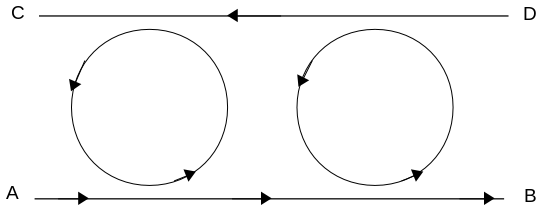
\includegraphics[width = \textwidth]{img/Asyina}
\caption{Asymptotic in field for channel $A$}
\end{subfigure}%
\begin{subfigure}{0.5\textwidth}
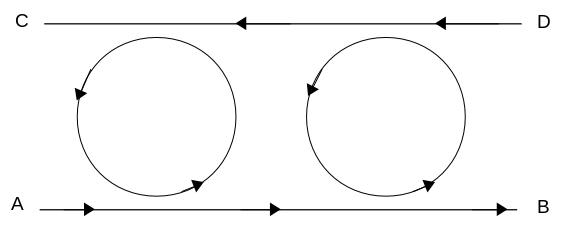
\includegraphics[width = \textwidth]{img/Asyoutb}
\caption{Asymptotic out field for channel $B$}
\end{subfigure}
\caption{Asymptotic fields for the coupled resonators, the ring on the left is identified as 1, while the ring on the right as 2}\label{asyfields}
\end{figure}

In this section we derive the explicit form of $S_{bb}$ and in analogy also for $S_{bc}$ and $S_{cc}$. Recall from equation \eqref{S}
\begin{multline}\label{sbb} S_{bb} =\frac{3}{2\varepsilon_0}\sqrt{\frac{(\hbar\omega_{k_1})(\hbar\omega_{k_2})(\hbar\omega_{k_3})(\hbar\omega_{k_4})}{16}}\cdot \\ \int d\r \Gamma^{ijkl}_3D^{i,asy-in}_{a,k_1}(\r)D^{j,asy-in}_{a,k_2}(\r)\left[D^{k,asy-out}_{b,k_3}(\r)\right]^*\left[D^{l,asy-out}_{b,k_4}(\r)\right]^*\end{multline}
in section \ref{section:asymptotic} we stated that the asympotic-in field associated with channel $A$ corresponds to a wave incoming in channel $A$ and outgoing waves in every channel, and similarly asymptotic-out field of channel $B$ consist of an outgoing wave in channel $B$ and incoming waves in the other channels. These asympotitic fields are depicted in figure \ref{asyfields}. The integral of $S_{bb}$ is performed in general over all the space, but outside waveguides and resonators the field is zero, futhermore, since the field inside the ring in enhanced with respect to the field in the waveguide, we can neglet the contribution of the field in the waveguides. Therefore the integration can be performed only over the rings. With this assumption we can write the asymptotic fields as
\[\mathbf{D}^{asy-in}_{a,k} \propto FE_{1a}(\omega) \mathbf{d}_1(\r_\perp)e^{ik_1z} + FE_{2a}(\omega) \mathbf{d}_2(\r_\perp)e^{ik_2z} \]
where $z$ is the coordinate in the counterclockwise direction along the rings circunference and $\r_\perp$ are the coordinates perpendicular to $z$. $FE_{1a}$ is the field enhancement of the first ring when the input wave is in channel $A$, while obviously $FE_{2a}$ refers to the second ring. Similarly the asymptotic-out field associated with channel $B$ can be written as
\[\mathbf{D}^{asy-out}_{a,k} \propto FE_{1b}(\omega) \mathbf{d}_1(\r_\perp)e^{ik_1z} + FE_{2b}(\omega) \mathbf{d}_2(\r_\perp)e^{ik_2z} \]
using the last two equations in \eqref{sbb} leads to a lot of terms, everyone associated with a specific physical interpretation. In particular every terms correspond to a possible path for the photons that are scattered in the channel $B$, for example, the annihilated pump photon can be both inside the first ring, or both in the second one or even one in the first ring, one in the second one. Same argument for the created photons that can be created both inside the first ring, both inside the second or one in each ring. The combination of these paths are represented by all terms in $S_{bb}$, however each of this terms are proportional to the field $\mathbf{d}_1(\r_{\perp})$ and $\mathbf{d}_1(\r_{\perp})$ that are non zero only inside the ring, therefore a term that contain a factor $\mathbf{d}_1(\r_{\perp})\mathbf{d}_2(\r_{\perp})$ is zero everywhere, because in the first ring the second factor is zero and in the second ring the first factor is zero. The only term that survive the integration are 
